% 
% Lecture Template for ME3050 -  Dynamics Modeling and Controls - Tennessee Technological University
%
% Spring 2020 - Summer 2020
% Tristan Hill, May 07, 2020 - June 12, 2020
% Module 5 - Rotating Systems
% Topic 1 - The Dynamics of Rotation
%

\documentclass{beamer}                         % for presentation (has nav buttons at bottom)
%\documentclass[handout]{beamer}  % for handout 
\usepackage{beamerthemesplit}
\usepackage{amsmath}
\usepackage{listings}
\usepackage{multicol}
\usepackage{framed}

\beamertemplateballitem

% custom colors
\definecolor{TTUpurple}{rgb}{0.3098, 0.1607, 0.5176} % TTU Purple (primary)
\definecolor{TTUgold}{rgb}{1.0000, 0.8666, 0.0000} % TTU Gold (primary) 
\definecolor{mygray}{rgb}{.6, .6, .6}
\definecolor{mypurple}{rgb}{0.6,0.1961,0.8}
\definecolor{mybrown}{rgb}{0.5451,0.2706,0.0745}
\definecolor{mygreen}{rgb}{0, .39, 0}
\definecolor{mypink}{rgb}{0.9960, 0, 0.9960}

% color commands
\newcommand{\R}{\color{red}}
\newcommand{\B}{\color{blue}}
\newcommand{\BR}{\color{mybrown}}
\newcommand{\K}{\color{black}}
\newcommand{\G}{\color{mygreen}}
\newcommand{\PR}{\color{mypurple}}
\newcommand{\PN}{\color{mypink}}
\newcommand{\OR}{\color{TTU}}
\newcommand{\GD}{\color{TTUgold}}


\setbeamercolor{palette primary}{bg=TTUpurple,fg=TTUgold}
\setbeamercolor{palette secondary}{bg=black,fg=TTUgold}
\setbeamercolor{palette tertiary}{bg=black,fg=TTUpurple}
\setbeamercolor{palette quaternary}{bg=TTUgold,fg=black}
\setbeamercolor{structure}{fg=TTUpurple} % itemize, enumerate, etc
\setbeamercolor{section in toc}{fg=TTUpurple} % TOC sections

%\usefonttheme{professionalfonts}

\newcommand{\Lagr}{\mathcal{L}} % lagrangian

\newcommand{\hspcu}{\underline{\hspace{20mm}}} % large horizontal space w underline
\newcommand{\vspccc}{\vspace{6mm}\\} % large vertical space
\newcommand{\vspcc}{\vspace{4mm}\\}   % medium vertical space
\newcommand{\vspc}{\vspace{2mm}\\}     % small vertical space

\newcommand{\hspcccc}{\hspace{10mm}} % large horizontal space
\newcommand{\hspccc}{\hspace{6mm}} % large horizontal space
\newcommand{\hspcc}{\hspace{4mm}}   % medium horizontal space
\newcommand{\hspc}{\hspace{2mm}}     % small horizontal space

\newcommand{\eqscl}{0.9}     % small horizontal space


\author{ME3050 - Dynamics Modeling and Controls} % original formatting from Mike Renfro, September 21, 2004

\newcommand{\MNUM}{5\hspace{2mm}} % Module number
\newcommand{\TNUM}{1\hspace{2mm}} % Topic number 
\newcommand{\moduletitle}{Rotation Systems }
\newcommand{\topictitle}{The Dynamics of Rotation} 

\newcommand{\sectiontitleI}{Newton's Second in Rotation}
\newcommand{\sectiontitleII}{Fixed Axis Rotation}
\newcommand{\sectiontitleIII}{Instantaneous Center of Rotation}
\newcommand{\sectiontitleIV}{Engineering Applications}

% custom box
\newsavebox{\mybox}

\title{Module \MNUM - \moduletitle}

\date{Mechanical Engineering\vspc Tennessee Technological University}

\begin{document}

\lstset{language=MATLAB,basicstyle=\ttfamily\small,showstringspaces=false}

\frame{\titlepage \center\begin{framed}\Large \textbf{Topic \TNUM - \topictitle}\end{framed} \vspace{5mm}}

% Section 0: Outline
\frame{

\large \textbf{Topic \TNUM - \topictitle} \vspace{3mm}\\

\begin{itemize}

	\item \sectiontitleI		\vspc % Section I
	\item \sectiontitleII 	\vspc % Section II
	\item \sectiontitleIII 	\vspc %Section III
	\item \sectiontitleIV 	\vspc %Section IV

\end{itemize}

}

% Section I:
\section{\sectiontitleI}

\frame{
\frametitle{\sectiontitleI}

 Newton's Second Law equates the mass moment of inertia to the angular acceleration of a rigid body. \vspc
 
 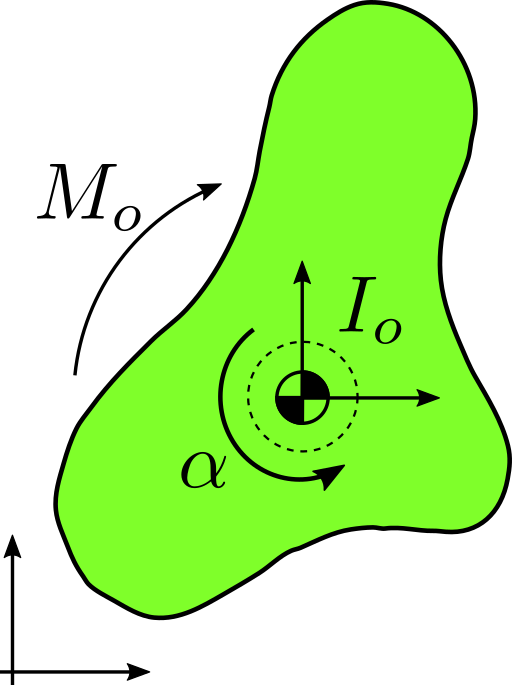
\includegraphics[scale=.225]{moment_inertia_fig5.png}  \hspcc \scalebox{1}{$\Sigma M_o = I_o \alpha = I_o \dot{\omega}$}\vspc



\vspace{1mm}
{\tiny Images: T.Hill}
}


% Section II:
\section{\sectiontitleII}

\frame{
\frametitle{\sectiontitleII}

This expression is only valid for a system constrained\\  to {\it rotation about a fixed axis}. \vspace{5mm}\\

 \hspace{10mm}
\includegraphics[scale=.25]{moment_inertia_fig8.png}  \hspcc \scalebox{1}{$\Sigma M_o = I_o \alpha = I_o \dot{\omega}$}\vspc

\vspace{15mm}
{\tiny Images: T.Hill}

}

% Section III:
\section{\sectiontitleIII}

\frame{
\frametitle{\sectiontitleIII}

As you know there is a kinetic energy associated with the rotating mass. If the rotation is in the vertical plane there is a gravitational potential. \vspc

 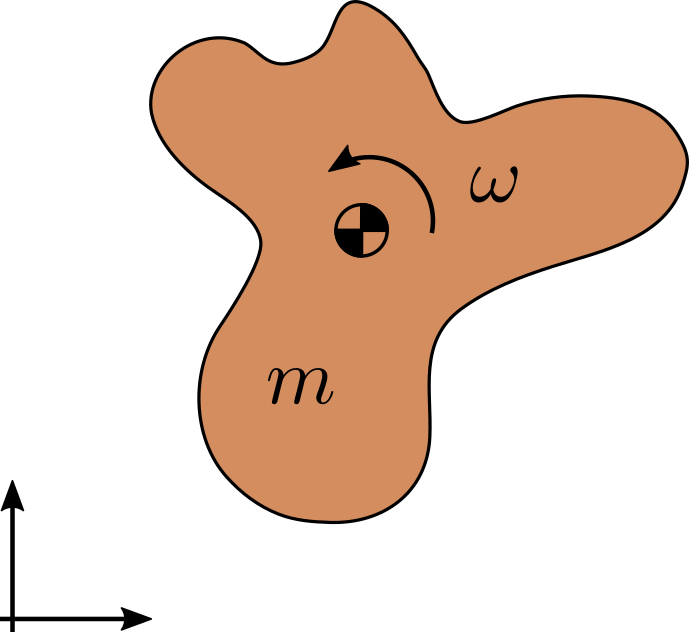
\includegraphics[scale=.225]{moment_inertia_fig6.png} \hspace{20mm}  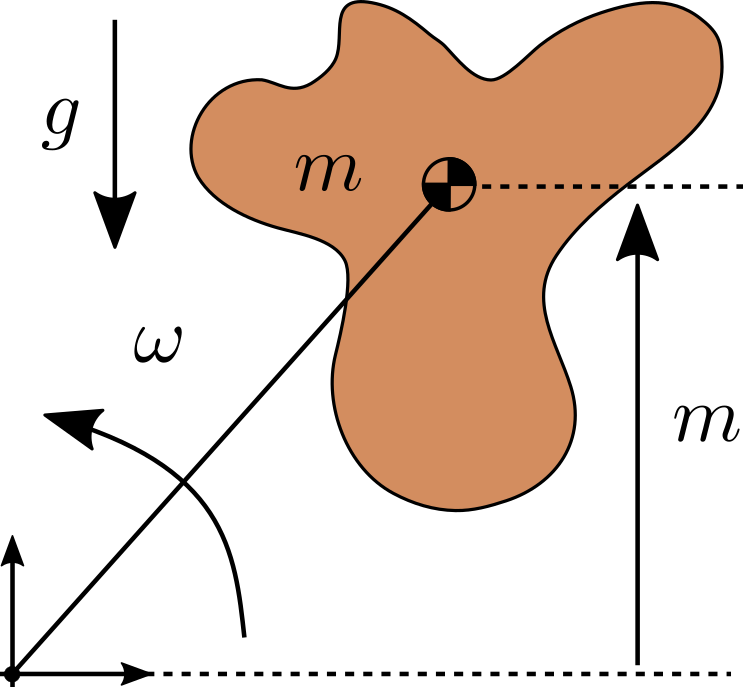
\includegraphics[scale=.225]{moment_inertia_fig7.png}  \vspc

\scalebox{1}{$KE  = T = \frac{1}{2}I_o\omega^2$} \hspace{25mm} \scalebox{1}{$PE  = V = mgy$}

}

% Section IV:
\section{\sectiontitleIV}

\frame{
\frametitle{\sectiontitleIV}

Rotating systems are used in machines and engineering systems of all types.\

\begin{itemize}

 	\item IC engines
 	
 	\item Electric Motors
 	
 	\item Wheels, Gears, Transmissions
 	
 	\item ...


\end{itemize}

}
	
\end{document}





